\chapter{অনুসন্ধানমূলক ডেটা বিশ্লেষণ}\label{ch:eda}

এই অধ্যায় বর্ণনামূলক প্রশ্ন, \emph{কী ঘটেছে?}, এর উত্তর দেয় এবং \emph{কেন} প্রশ্নের উত্তর দেওয়া শুরু করে। সব ফলাফল
\texttt{eda.py} দিয়ে পূর্ণ পরিষ্কার ডেটাসেটে হিসাব করা।

\section{সামগ্রিক কর্মদক্ষতা ও প্রবৃদ্ধি}
পুরো সময়কালে কোম্পানি \NRows টি অর্ডারে \TotalUnits মিলিয়ন ইউনিট বিক্রি করেছে, যার নিট বিক্রয়মূল্য \TotalSales মিলিয়ন টাকা।
গড় অর্ডারের মূল্য ছিল \AOV টাকা, এবং ডিসকাউন্ট গড়ে মোট মূল্যের \AvgDiscount\%, যার মোট খরচ \DiscountCost মিলিয়ন টাকা।
\Cref{tab:annual} ও \cref{fig:trend} স্থির প্রবৃদ্ধি দেখায়। প্রথম ও শেষ পূর্ণ বছরের মধ্যে (2020--2025) নিট বিক্রয় বছরে
\CAGRSales\% চক্রবৃদ্ধি হারে বেড়েছে, এবং জানুয়ারি--সেপ্টেম্বর 2026-এর বিক্রয় 2025-এর একই মাসগুলোর তুলনায় \YTDGrowth\% বেশি।

\begin{table}[htbp]
\centering
\small
\caption{বার্ষিক কর্মদক্ষতার সারসংক্ষেপ, 2020--2026}
\label{tab:annual}
\begin{adjustbox}{max width=\linewidth}
\begin{tabular}{lrrrrrrr}
\toprule
\textbf{Year} & \textbf{Orders} & \textbf{Units} & \textbf{Net sales (BDT M)} & \textbf{AOV (BDT)} & \textbf{Avg price} & \textbf{Disc. \%} & \textbf{YoY \%} \\
\midrule
2020 & 74,788 & 398,005 & 28.62 & 382.7 & 72.0 & 2.34 & -- \\
2021 & 73,636 & 418,104 & 37.02 & 502.7 & 88.6 & 2.35 & +29.3 \\
2022 & 73,898 & 440,150 & 41.00 & 554.8 & 93.4 & 2.34 & +10.8 \\
2023 & 73,598 & 460,465 & 46.17 & 627.3 & 100.5 & 2.36 & +12.6 \\
2024 & 74,282 & 486,293 & 53.03 & 713.9 & 109.8 & 2.35 & +14.9 \\
2025 & 74,442 & 507,262 & 61.78 & 829.9 & 122.3 & 2.35 & +16.5 \\
2026* & 55,356 & 381,678 & 50.75 & 916.8 & 133.8 & 2.34 & -- \\
\bottomrule
\end{tabular}
\end{adjustbox}
\par\smallskip\parbox{0.92\linewidth}{\footnotesize\emph{টীকা:} * 2026 সালে কেবল জানুয়ারি--সেপ্টেম্বর অন্তর্ভুক্ত, তাই এর প্রবৃদ্ধি হিসাব করা হয়নি। AOV = গড় অর্ডার-মূল্য; Avg price = গড় একক বিক্রয়মূল্য।}
\end{table}

\begin{figure}[htbp]\centering
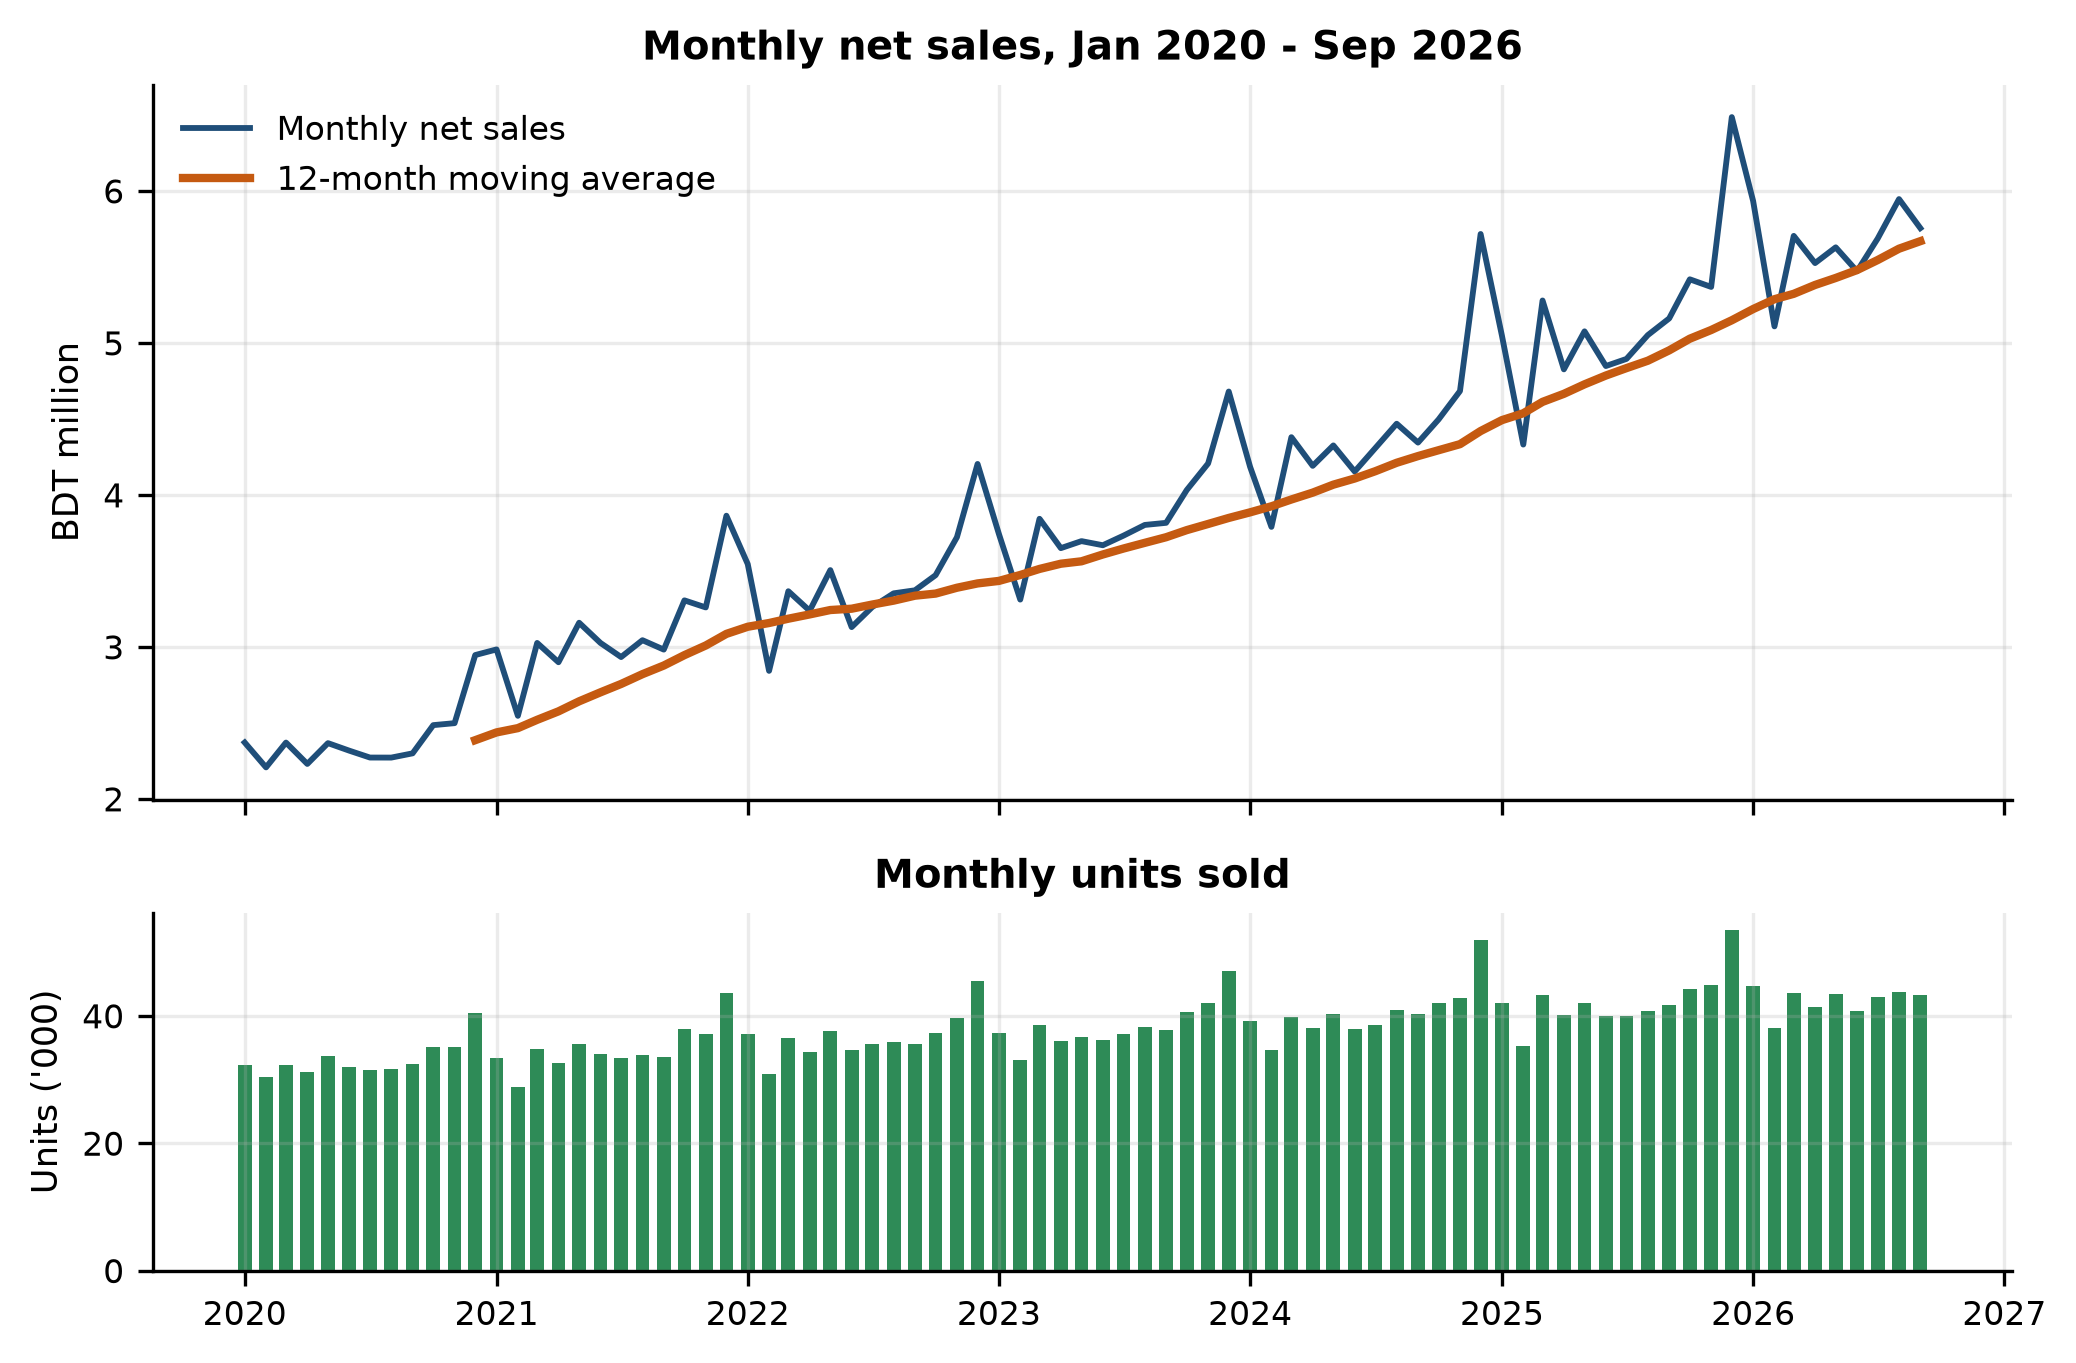
\includegraphics[width=\linewidth]{eda_monthly_trend}
\caption{মাসিক নিট বিক্রয় ও 12-মাসের চলমান গড় (উপরে) এবং মাসিক বিক্রীত ইউনিট (নিচে)}\label{fig:trend}
\end{figure}

\subsection{প্রবৃদ্ধি কোথা থেকে আসে?}
ইউনিট বেড়েছে বছরে মাত্র \CAGRUnits\%, অথচ গড় বিক্রয়মূল্য বেড়েছে বছরে \CAGRPrice\%। বিক্রয় প্রবৃদ্ধিকে হুবহু বিভাজন করা যায়:
$(1+g_{\text{sales}}) = (1+g_{\text{volume}})(1+g_{\text{price}})$। \Cref{tab:pricevolume} ও \cref{fig:pricevolume} দেখায় যে গড়ে
বার্ষিক প্রবৃদ্ধির প্রায় \AvgVolGrowth শতাংশ-বিন্দু এসেছে পরিমাণ থেকে এবং \AvgPriceGrowth এসেছে মূল্য ও পণ্য-মিশ্রণ থেকে। 2021-এর
ব্যতিক্রমী বৃদ্ধি বেশি দামের গিফট বক্স চালুর সঙ্গে মিলে যায় (একটি মিশ্রণ-প্রভাব); পরের বছরগুলো নিয়মিত তালিকা-মূল্য বৃদ্ধির প্রতিফলন।
ব্যবস্থাপনার জন্য এই পার্থক্য গুরুত্বপূর্ণ: মূল্য-নির্ভর প্রবৃদ্ধি অনির্দিষ্টকাল চলতে পারে না, একসময় তা ভোক্তার ক্রয়-সামর্থ্যের সীমায় পৌঁছায়।

\begin{table}[htbp]
\centering
\small
\caption{বার্ষিক বিক্রয় প্রবৃদ্ধির পরিমাণ (volume) ও মূল্য (price) প্রভাবে বিভাজন}
\label{tab:pricevolume}
\begin{adjustbox}{max width=\linewidth}
\begin{tabular}{lrrr}
\toprule
\textbf{Year} & \textbf{Sales growth \%} & \textbf{Volume growth \%} & \textbf{Avg price growth \%} \\
\midrule
2021 & +29.3 & +5.0 & +23.1 \\
2022 & +10.8 & +5.3 & +5.2 \\
2023 & +12.6 & +4.6 & +7.6 \\
2024 & +14.9 & +5.6 & +8.8 \\
2025 & +16.5 & +4.3 & +11.7 \\
\bottomrule
\end{tabular}
\end{adjustbox}
\par\smallskip\parbox{0.92\linewidth}{\footnotesize\emph{টীকা:} $(1+g_{sales}) = (1+g_{volume})(1+g_{price})$; এখানে মূল্য মানে ইউনিটপ্রতি নিট আয়, তাই এতে পণ্য-মিশ্রণের পরিবর্তনও প্রতিফলিত।}
\end{table}

\begin{figure}[htbp]\centering
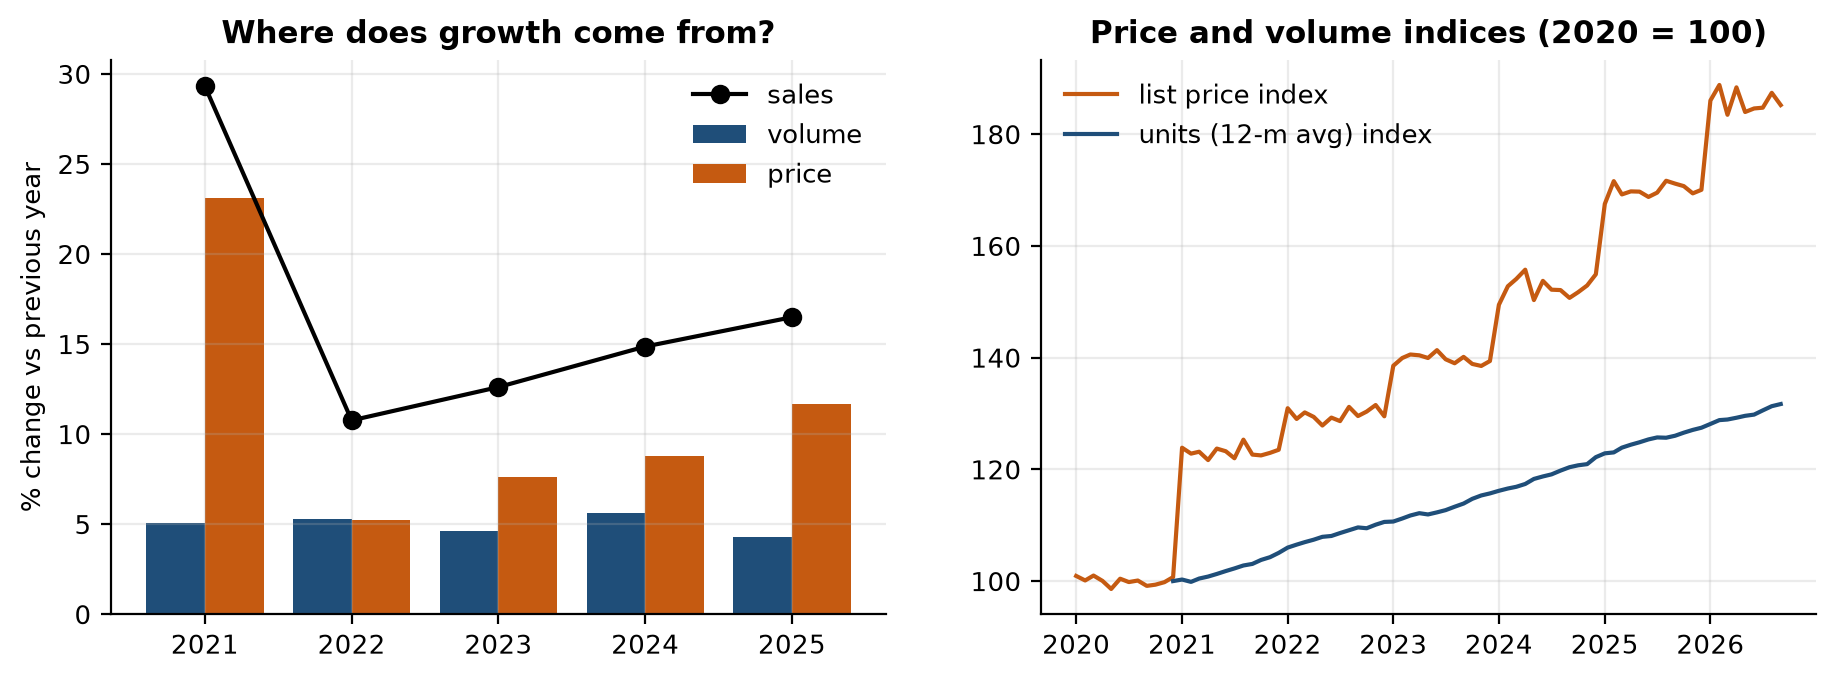
\includegraphics[width=\linewidth]{eda_price_volume}
\caption{প্রবৃদ্ধির বিভাজন (বামে) এবং মূল্য বনাম পরিমাণ সূচক (ডানে)}\label{fig:pricevolume}
\end{figure}

\subsection{চাহিদা কি মূল্য-সংবেদনশীল?}
মূল্যের প্রভাবকে সাধারণ প্রবৃদ্ধি থেকে আলাদা করতে পণ্য-মাস প্যানেলে একটি fixed-effects রিগ্রেশন দিয়ে চাহিদার মূল্য-স্থিতিস্থাপকতা
নির্ণয় করা হয়েছে:
\[
  \log(\text{units}_{pt}) = \beta \log(\text{price}_{pt}) + \alpha_p + \gamma_{\text{year}(t)} + \delta_{\text{month}(t)} + \varepsilon_{pt}.
\]
পণ্য-প্রভাব $\alpha_p$ পণ্যগুলোর আকারের পার্থক্য, বছর-প্রভাব সাধারণ বাজার-প্রবৃদ্ধি এবং মাস-প্রভাব মৌসুমিতা শোষণ করে। নির্ণীত
স্থিতিস্থাপকতা $\hat\beta = \Elasticity$, 95\% আস্থা-ব্যবধান \ElasticityLo থেকে \ElasticityHi (robust standard error;
$p = \ElasticityP$; $R^2 = \ElasticityRtwo$)। এটি শূন্য থেকে তাৎপর্যপূর্ণভাবে আলাদা নয়, অর্থাৎ পর্যবেক্ষিত সীমার মধ্যে চাহিদা
\emph{মূল্য-অস্থিতিস্থাপক}। বছর-প্রভাব ছাড়া একটি সরল রিগ্রেশন বিভ্রান্তিকর \emph{ধনাত্মক} স্থিতিস্থাপকতা (\ElasticityNaive) দেয়,
কারণ সময়ের সঙ্গে মূল্য ও পরিমাণ দুটোই বেড়েছে। এটি confounding-এর একটি পাঠ্যপুস্তকীয় উদাহরণ, এবং এ কারণেই ব্যাখ্যামূলক মডেল
সতর্কভাবে নির্দিষ্ট করতে হয় \citep{shmueli2010}।

\section{মৌসুমিতা ও ক্যালেন্ডারের প্রভাব}
বিক্রয়ে একটি স্পষ্ট বার্ষিক চক্র রয়েছে (\cref{fig:seasonality})। ডিসেম্বর সবচেয়ে শক্তিশালী মাস, মৌসুমি সূচক \PeakIndex
(গড় মাস = 100); অক্টোবর (\OctIndex) ও নভেম্বরও (\NovIndex) গড়ের উপরে, যা বছর-শেষের উৎসব ও উপহারের মৌসুমের সঙ্গে সামঞ্জস্যপূর্ণ।
ফেব্রুয়ারি সবচেয়ে দুর্বল (\TroughIndex)। ফেব্রুয়ারির দুর্বলতার একটি অংশ কেবল এর কম দিনসংখ্যার কারণে: প্রতি কর্মদিবস হিসেবে এর সূচক
\FebPerDay, অথচ ডিসেম্বরের প্রতিদিনের সূচক উচ্চই থাকে (\DecPerDay)। প্রবণতা-মুক্ত দৈনিক বিক্রয়ে Kruskal--Wallis টেস্ট নিশ্চিত করে যে
ক্যালেন্ডারের মাস গুরুত্বপূর্ণ ($H = \KWMonthH$, $p<0.001$)। বিপরীতে সপ্তাহের দিনের প্রভাব প্রায় নেই: সপ্তাহের দিনগুলোর গড় দৈনিক
বিক্রয়ের coefficient of variation মাত্র \DowCV\%।

\begin{figure}[htbp]\centering
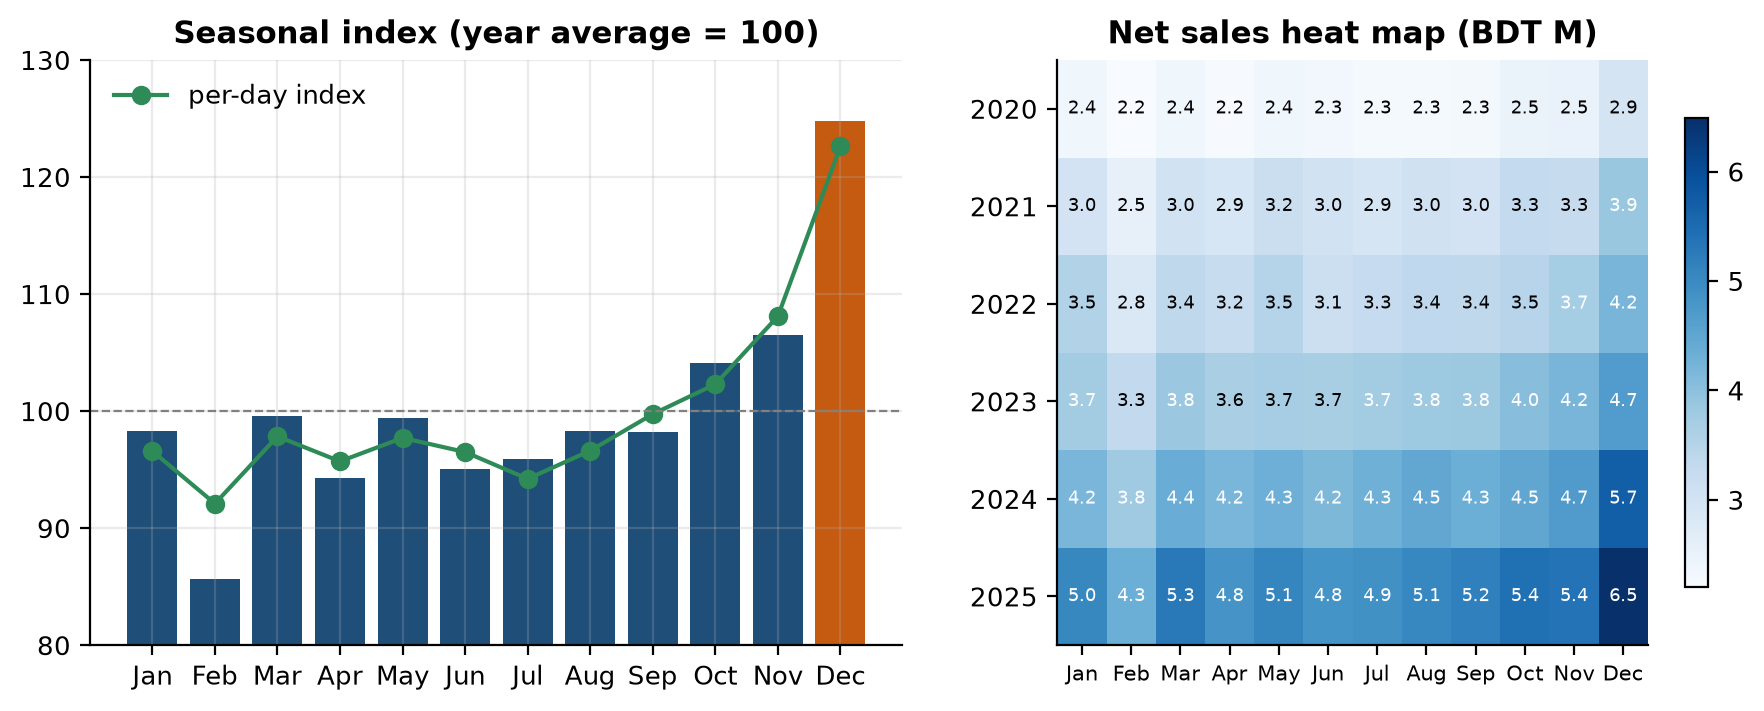
\includegraphics[width=\linewidth]{eda_seasonality}
\caption{মাস অনুযায়ী মৌসুমি সূচক (বামে) এবং বছর $\times$ মাস অনুযায়ী নিট বিক্রয়ের heat map (ডানে)}\label{fig:seasonality}
\end{figure}

\section{পণ্য ও ক্যাটাগরি}
\Cref{tab:category} ও \cref{fig:pareto} ক্যাটাগরি-কাঠামো দেখায়। \TopCategory সবচেয়ে বড় ক্যাটাগরি (বিক্রয়ের \TopCategoryShare\%),
এরপর Pound Cake ও Swiss Roll। Layer Cake-এর প্রবৃদ্ধির হার সর্বোচ্চ (বছরে \FastCategoryCAGR\%), যা মূলত 2021-এ যুক্ত গিফট-বক্স
সংস্করণ থেকে এসেছে; এটি মনে করিয়ে দেয় যে ক্যাটাগরির প্রবৃদ্ধিতে স্বাভাবিক প্রবৃদ্ধি ও পণ্য-পরিসর পরিবর্তন মিশে থাকে। Pareto বিশ্লেষণ
\NProducts টি পণ্যকে ভাগ করে \NClassA টি A-শ্রেণির পণ্যে (যারা আয়ের 80\% আনে), \NClassB টি B-শ্রেণি ও \NClassC টি C-শ্রেণিতে।
সর্বাধিক বিক্রীত দশটি পণ্যই নিট বিক্রয়ের \TopTenShare\% দেয় (\cref{tab:topproducts})।

\begin{table}[htbp]
\centering
\small
\caption{পণ্য-ক্যাটাগরি অনুযায়ী আয় ও প্রবৃদ্ধি}
\label{tab:category}
\begin{adjustbox}{max width=\linewidth}
\begin{tabular}{lrrrr}
\toprule
\textbf{Category} & \textbf{Net sales (BDT M)} & \textbf{Share \%} & \textbf{Products} & \textbf{CAGR 2020-25 \%} \\
\midrule
Muffin & 71.47 & 22.4 & 9 & +32.3 \\
Pound Cake & 61.76 & 19.4 & 12 & +9.7 \\
Swiss Roll & 38.81 & 12.2 & 4 & +9.6 \\
Fruit Cake & 28.90 & 9.1 & 5 & +9.9 \\
Layer Cake & 28.47 & 8.9 & 4 & +67.7 \\
Dry Cake & 25.59 & 8.0 & 3 & +9.4 \\
Cookie & 21.72 & 6.8 & 3 & +11.0 \\
Plain Cake & 16.57 & 5.2 & 6 & +10.4 \\
Velvet Cake & 11.75 & 3.7 & 1 & +10.3 \\
Classic Brownie & 6.27 & 2.0 & 1 & +10.8 \\
Premium & 4.02 & 1.3 & 1 & -- \\
Breakfast & 1.75 & 0.6 & 1 & -- \\
Bread & 1.28 & 0.4 & 2 & -- \\
\bottomrule
\end{tabular}
\end{adjustbox}
\par\smallskip\parbox{0.92\linewidth}{\footnotesize\emph{টীকা:} CAGR প্রথম ও শেষ পূর্ণ বছরের মধ্যে হিসাবকৃত। 2020-এর পরে চালু হওয়া ক্যাটাগরির প্রবৃদ্ধি তাদের চালুর বছর থেকে হিসাব করা।}
\end{table}
\begin{table}[htbp]
\centering
\small
\caption{নিট বিক্রয় অনুযায়ী শীর্ষ দশটি পণ্য (Pareto/ABC বিশ্লেষণ)}
\label{tab:topproducts}
\begin{adjustbox}{max width=\linewidth}
\begin{tabular}{lrrr}
\toprule
\textbf{Product} & \textbf{Net sales (BDT M)} & \textbf{Cumulative share \%} & \textbf{Class} \\
\midrule
MUF007 Cappuccino Muffin Gift Pack & 15.41 & 4.8 & A \\
MUF006 Vanilla Muffin Gift Box & 12.48 & 8.8 & A \\
LAY004 Vanilla Layer Cake Gift Box & 12.44 & 12.7 & A \\
LAY002 Chocolate Layer Cake Gift Box & 12.29 & 16.5 & A \\
MUF003 Chocolate Muffin Gift Box & 12.25 & 20.4 & A \\
MUF009 Chocochips Muffin & 11.99 & 24.1 & A \\
MUF008 Raisin Muffin & 11.80 & 27.8 & A \\
VEL001 Chocolate Velvet Cake & 11.75 & 31.5 & A \\
SWR002 Chocolate Swiss Roll & 11.68 & 35.2 & A \\
SWR004 Strawberry Swiss Roll & 10.44 & 38.5 & A \\
\bottomrule
\end{tabular}
\end{adjustbox}
\end{table}

\begin{figure}[htbp]\centering
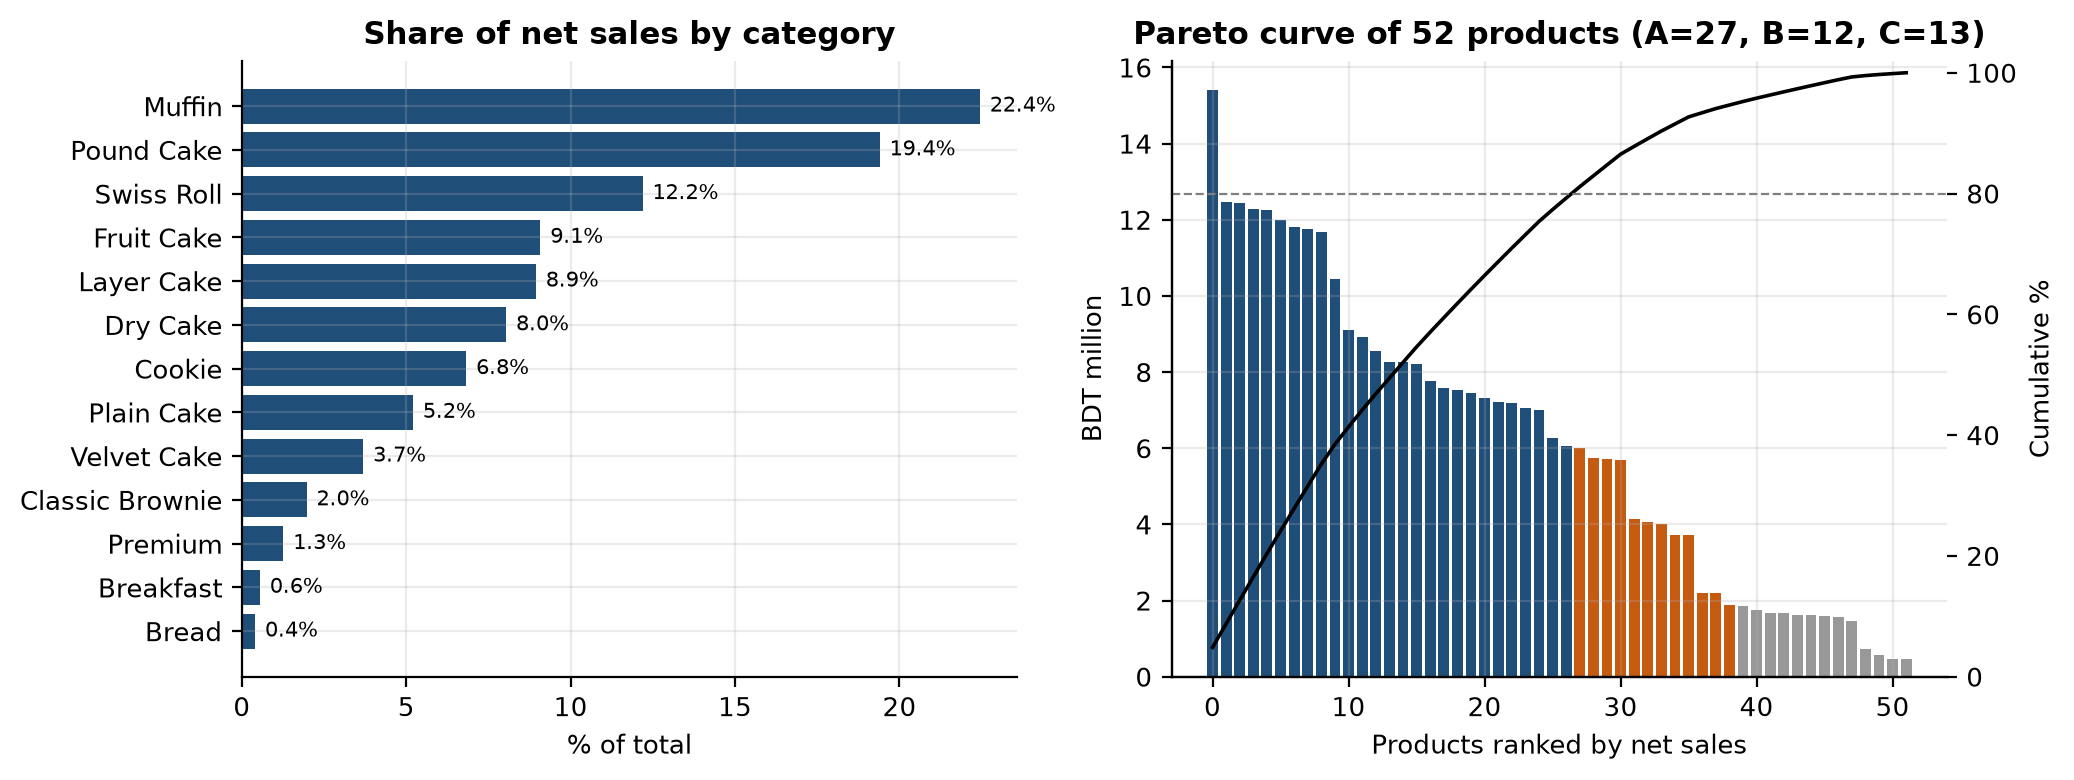
\includegraphics[width=\linewidth]{eda_category_pareto}
\caption{ক্যাটাগরি অনুযায়ী নিট বিক্রয়ের অংশ (বামে) এবং পণ্যের Pareto বক্ররেখা (ডানে)}\label{fig:pareto}
\end{figure}

\section{অঞ্চল, চ্যানেল ও গ্রাহক}
বিক্রয় ভৌগোলিকভাবে কেন্দ্রীভূত। ঢাকা একাই নিট বিক্রয়ের \DhakaShare\% আনে, আর ঢাকা ও চট্টগ্রাম মিলে \DhakaCtgShare\%
(\cref{tab:segments})। General Trade প্রধান চ্যানেল (\GTShare\%), এরপর Modern Trade (\MTShare\%), Distributor (\DistShare\%) ও
E-commerce (\EcomShare\%)। চ্যানেলভেদে অর্ডারের আকারে বড় পার্থক্য: একটি ডিস্ট্রিবিউটর অর্ডারে গড়ে \DistQty ইউনিট, E-commerce অর্ডারে
\EcomQty, General Trade-এ \GTQty এবং Modern Trade-এ \MTQty (\cref{fig:regionchannel})। অন্যদিকে গ্রাহকের ধরন অর্ডারের আকারে কোনো
পার্থক্য আনে না (Kruskal--Wallis $p=\PCustType$), এবং গ্রাহকের ধরনভেদে গড় অর্ডার-মূল্য প্রায় অভিন্ন। অর্থাৎ অর্ডারের আকার নির্ধারণ করে
\emph{বাজারে পৌঁছানোর পথ}, গ্রাহক কে তা নয়।

\begin{table}[htbp]
\centering
\footnotesize
\caption{অঞ্চল, চ্যানেল ও গ্রাহকের ধরন অনুযায়ী কর্মদক্ষতা}
\label{tab:segments}
\begin{adjustbox}{max width=\linewidth}
\begin{tabular}{llrrrrr}
\toprule
\textbf{Dimension} & \textbf{Level} & \textbf{Net sales (BDT M)} & \textbf{Share \%} & \textbf{Orders} & \textbf{AOV (BDT)} & \textbf{Units/order} \\
\midrule
Region & Dhaka & 139.76 & 43.9 & 169,661 & 823.8 & 7.85 \\
Region & Chattogram & 45.89 & 14.4 & 70,440 & 651.4 & 6.33 \\
Region & Gazipur & 25.74 & 8.1 & 39,853 & 645.9 & 6.34 \\
Region & Narayanganj & 21.23 & 6.7 & 35,195 & 603.1 & 5.93 \\
Region & Cumilla & 15.71 & 4.9 & 29,911 & 525.2 & 5.19 \\
Region & Sylhet & 15.27 & 4.8 & 29,901 & 510.6 & 4.92 \\
Region & Rangpur & 12.23 & 3.8 & 30,012 & 407.6 & 4.16 \\
Region & Rajshahi & 12.03 & 3.8 & 25,152 & 478.2 & 4.79 \\
Region & Khulna & 11.73 & 3.7 & 25,094 & 467.3 & 4.71 \\
Region & Mymensingh & 10.76 & 3.4 & 24,849 & 432.9 & 4.34 \\
Region & Barishal & 8.04 & 2.5 & 19,932 & 403.2 & 3.96 \\
Channel & General Trade & 145.21 & 45.6 & 260,431 & 557.6 & 5.32 \\
Channel & Modern Trade & 81.55 & 25.6 & 124,619 & 654.4 & 6.28 \\
Channel & Distributor & 72.90 & 22.9 & 64,861 & 1,123.9 & 11.43 \\
Channel & E-commerce & 18.72 & 5.9 & 50,089 & 373.7 & 3.66 \\
Customer type & Retailer & 143.28 & 45.0 & 224,582 & 638.0 & 6.19 \\
Customer type & Super Shop & 63.31 & 19.9 & 100,073 & 632.7 & 6.16 \\
Customer type & Distributor & 47.91 & 15.0 & 75,413 & 635.3 & 6.19 \\
Customer type & Online Customer & 31.95 & 10.0 & 49,759 & 642.0 & 6.17 \\
Customer type & Corporate & 31.93 & 10.0 & 50,173 & 636.4 & 6.21 \\
\bottomrule
\end{tabular}
\end{adjustbox}
\end{table}

\begin{figure}[htbp]\centering
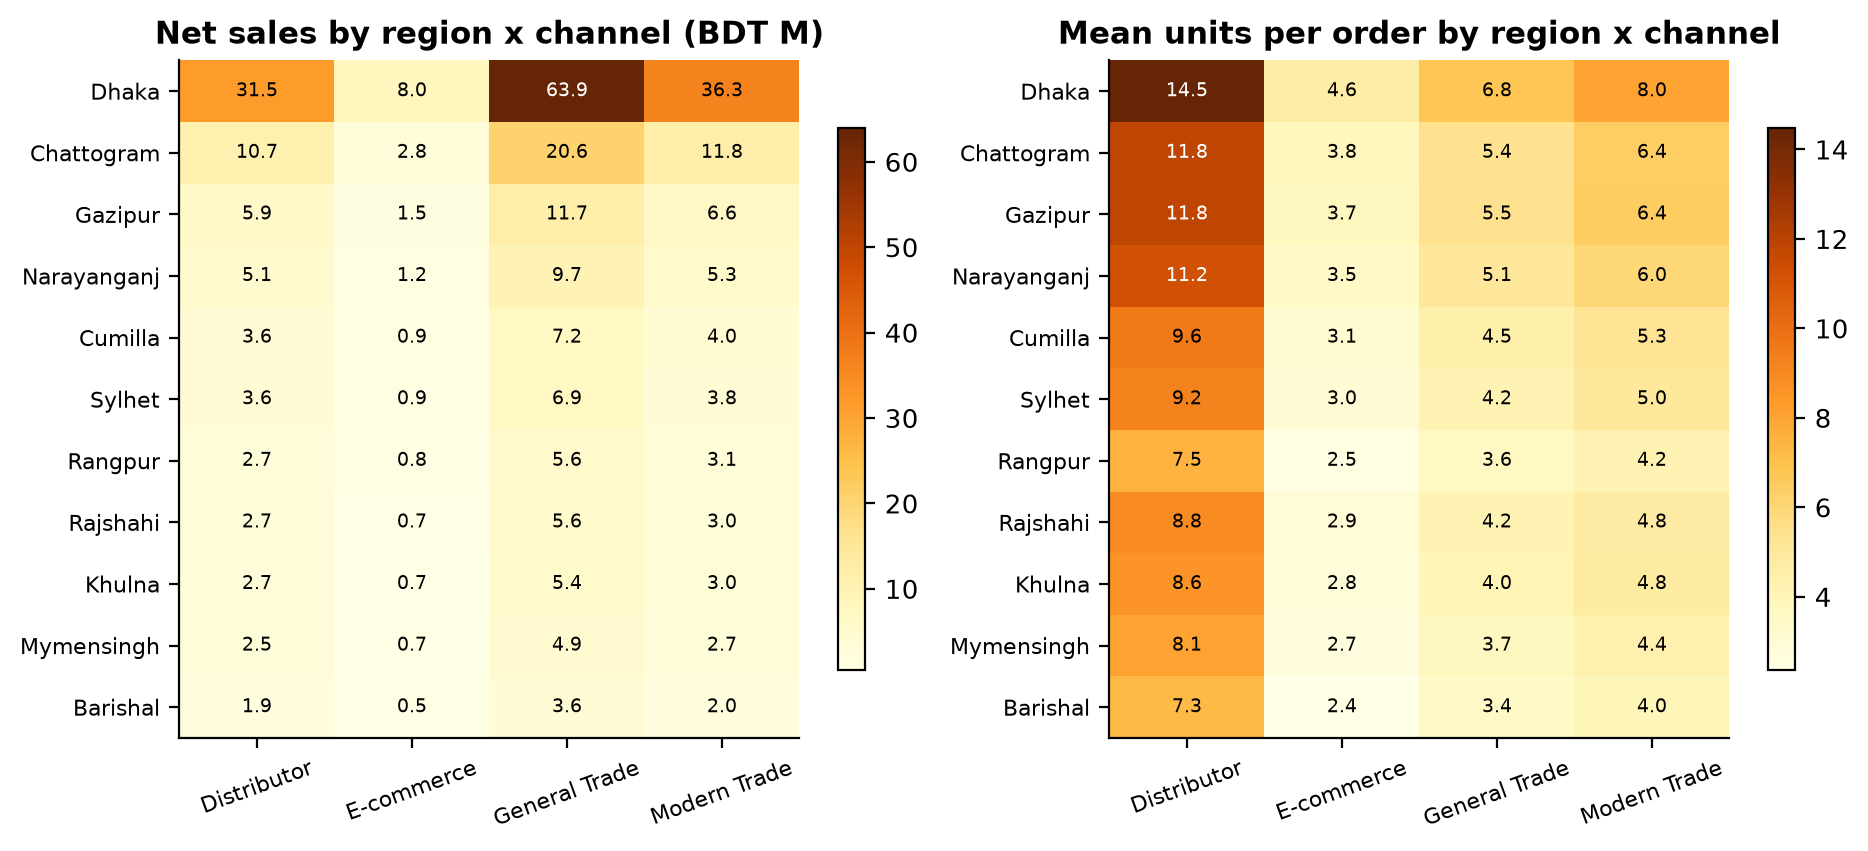
\includegraphics[width=\linewidth]{eda_region_channel}
\caption{অঞ্চল ও চ্যানেল অনুযায়ী নিট বিক্রয় (বামে) এবং অর্ডারপ্রতি গড় ইউনিট (ডানে)}\label{fig:regionchannel}
\end{figure}

\section{বণ্টন ও সম্পর্ক}
অর্ডারের পরিমাণ ও অর্ডার-মূল্য তীব্রভাবে ডানদিকে বিষম, skewness যথাক্রমে \QtySkew ও \ValueSkew (\cref{fig:distributions}):
অধিকাংশ অর্ডার ছোট, এবং বাল্ক অর্ডারের একটি দীর্ঘ লেজ আছে। এই আকৃতিই বিশ্লেষণ জুড়ে median, rank-ভিত্তিক টেস্ট ও log রূপান্তর
ব্যবহারের যৌক্তিকতা দেয়। Spearman সম্পর্ক-ম্যাট্রিক্স (\cref{fig:correlation}) দেখায় যে অর্ডার-মূল্য পরিমাণ ($\rho=\CorrSalesQty$) ও
মূল্য ($\rho=\CorrSalesPrice$) উভয় দিয়েই চালিত, কিন্তু পরিমাণ ও মূল্য কার্যত সম্পর্কহীন ($\rho=\CorrQtyPrice$): গ্রাহকরা বেশি দামের
পণ্যের কম প্যাক কেনেন না।

\begin{figure}[htbp]\centering
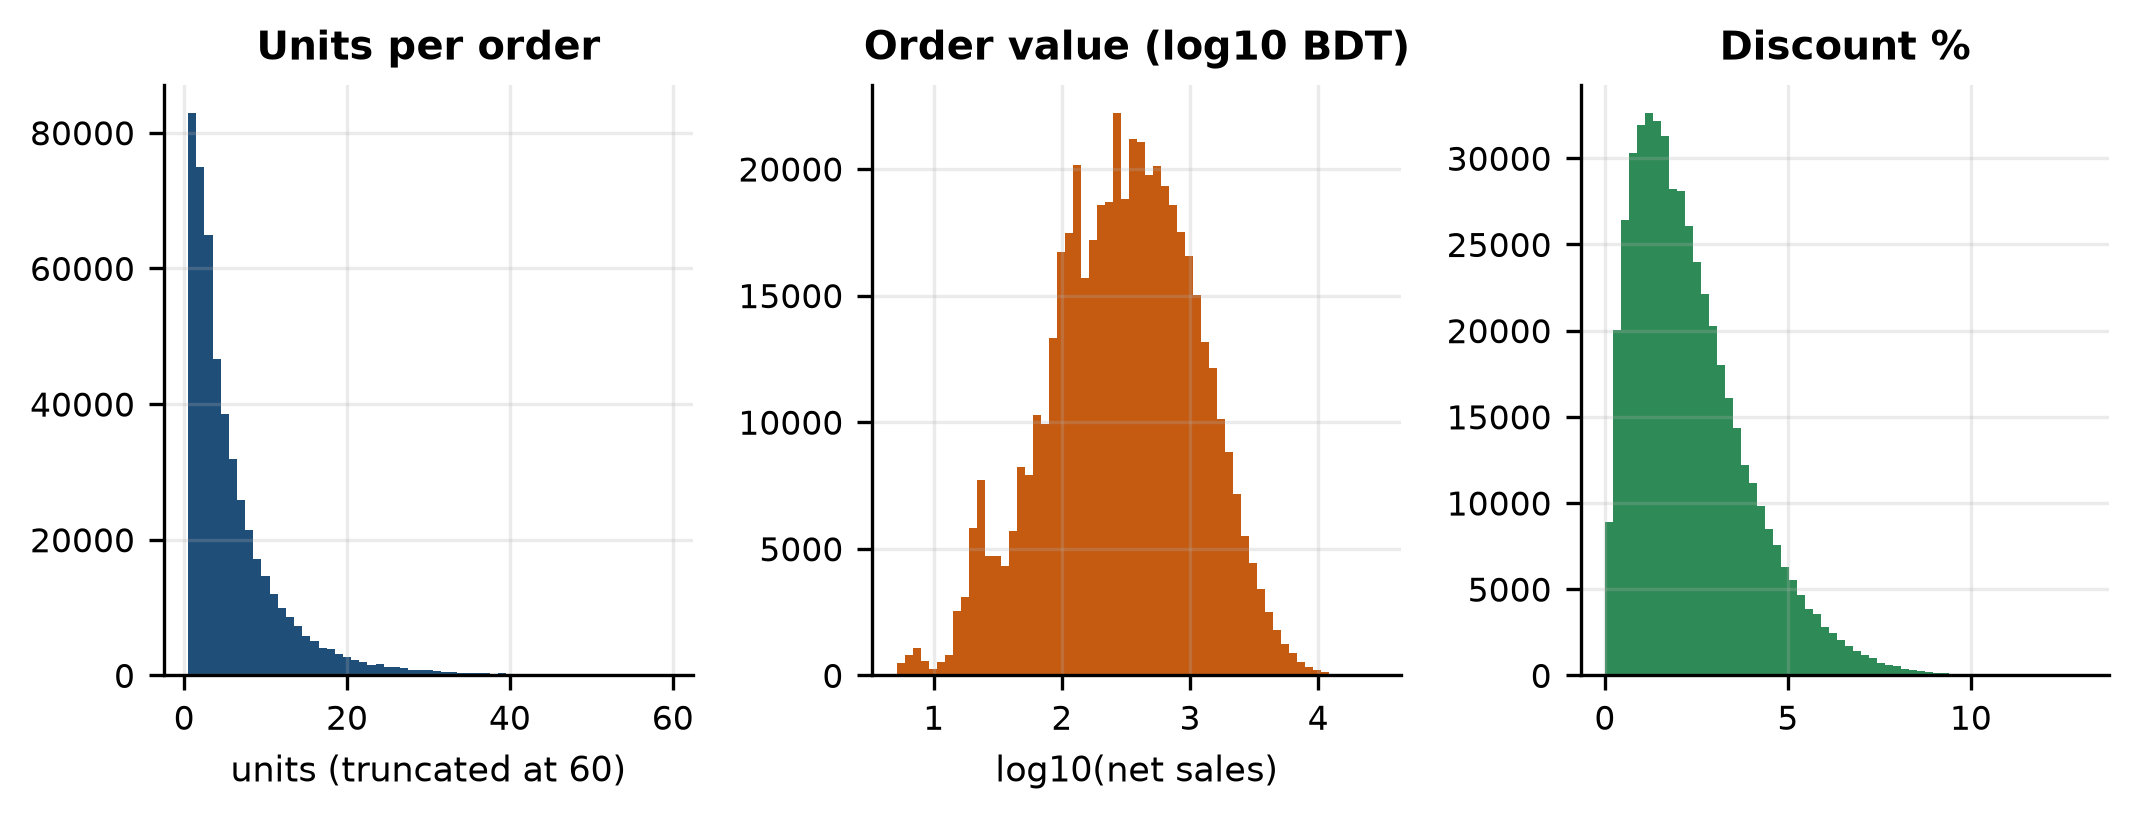
\includegraphics[width=\linewidth]{eda_distributions}
\caption{অর্ডারপ্রতি ইউনিট, অর্ডার-মূল্য (log স্কেল) ও ডিসকাউন্টের বণ্টন}\label{fig:distributions}
\end{figure}

\begin{figure}[htbp]\centering
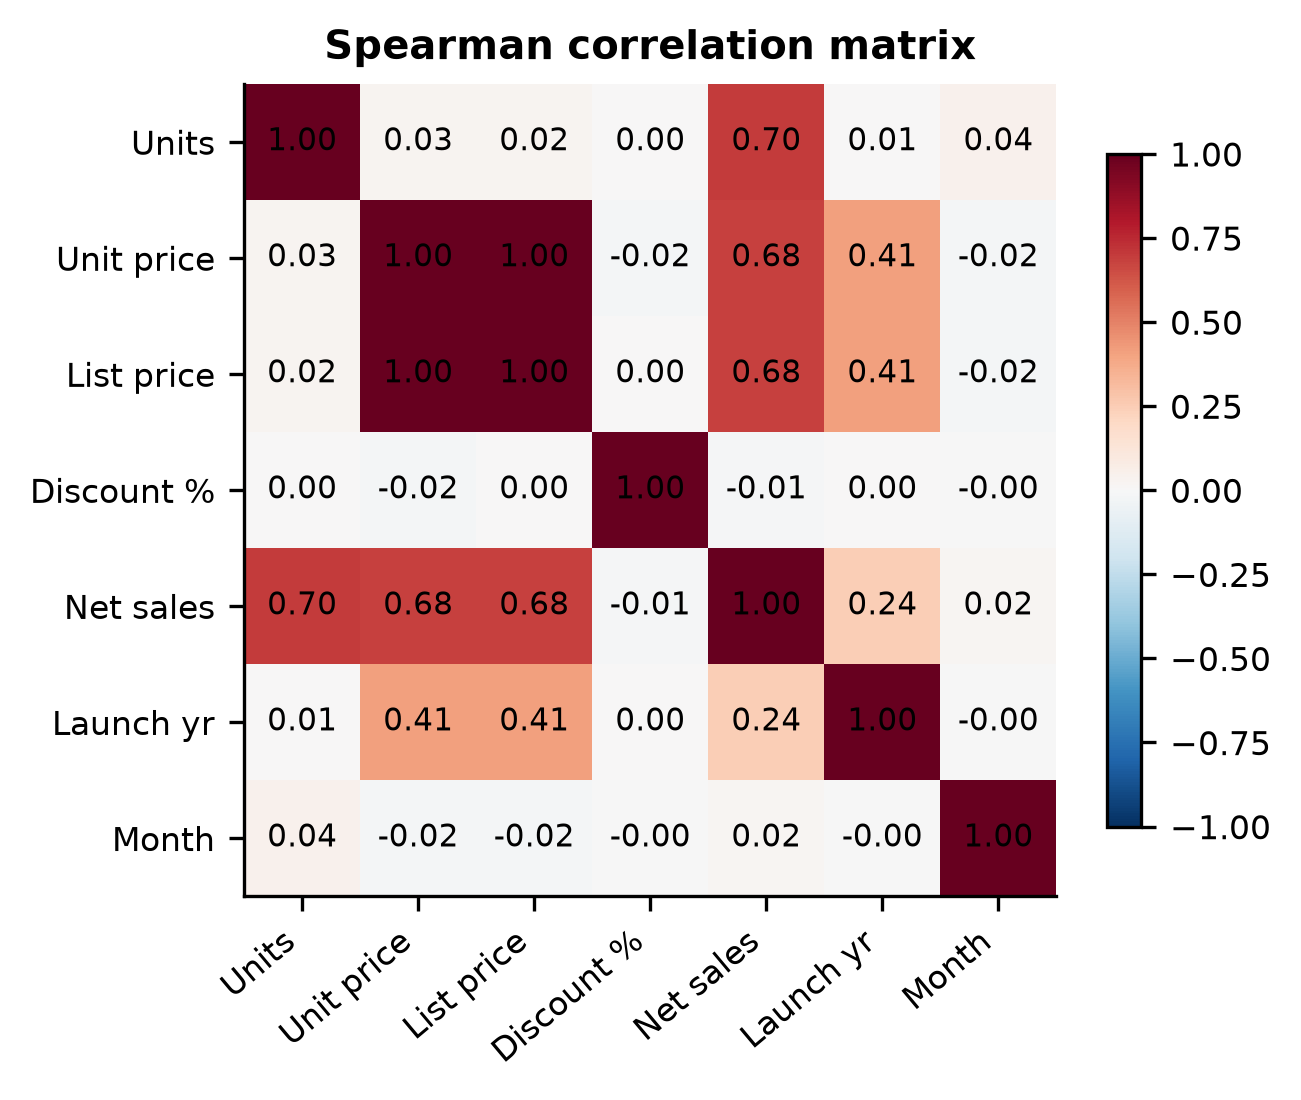
\includegraphics[width=.62\linewidth]{eda_correlation}
\caption{প্রধান সংখ্যাসূচক চলকগুলোর Spearman সম্পর্ক-ম্যাট্রিক্স}\label{fig:correlation}
\end{figure}

\section{হাইপোথিসিস টেস্ট}
\Cref{tab:tests} প্রধান অনুসন্ধানমূলক ফলাফলগুলোকে আনুষ্ঠানিক রূপ দেয়। পাঁচ লক্ষ পর্যবেক্ষণে দুটি বাদে সব পার্থক্যই পরিসংখ্যানিকভাবে
তাৎপর্যপূর্ণ, তাই ব্যাখ্যার জন্য effect size অপরিহার্য। অর্ডারের আকারের সবচেয়ে বেশি পরিবর্তন ব্যাখ্যা করে চ্যানেল
($\varepsilon^2=\EpsChannel$), তারপর অঞ্চল ($\varepsilon^2=\EpsRegion$)। চ্যানেল ও বড় অর্ডারের সম্পর্ক মাঝারি (Cram\'er's
$V=\CramerV$)। ডিসকাউন্টের গভীরতা ও অর্ডারের আকার \emph{সম্পর্কহীন} ($\rho=\RhoDisc$, $p=\PDisc$): প্রদত্ত ডিসকাউন্ট বড় কেনাকাটায়
উৎসাহ দেয় বলে মনে হয় না। এটি একটি সম্ভাব্য মূল্যবান ফলাফল, কারণ এই সময়কালে ডিসকাউন্টে কোম্পানির খরচ হয়েছে \DiscountCost মিলিয়ন টাকা।

\begin{table}[htbp]
\centering
\small
\caption{প্রধান অনুসন্ধানমূলক হাইপোথিসিসের পরিসংখ্যানিক টেস্ট}
\label{tab:tests}
\begin{adjustbox}{max width=\linewidth}
\begin{tabular}{llrrr}
\toprule
\textbf{Hypothesis (H0: no difference)} & \textbf{Test} & \textbf{Statistic} & \textbf{p-value} & \textbf{Effect size} \\
\midrule
Units/order by channel & Kruskal-Wallis & 43,269.88 & <0.001 & 0.0865 \\
Units/order by region & Kruskal-Wallis & 27,261.36 & <0.001 & 0.0545 \\
Units/order by customer type & Kruskal-Wallis & 2.62 & 0.623 & -0.0000 \\
Daily sales by month (detrended) & Kruskal-Wallis & 510.92 & <0.001 & 0.2293 \\
Discount \% vs units/order & Spearman rho & 0.00 & 0.479 & 0.0000 \\
Large order vs channel & Chi-square & 31,777.06 & <0.001 & 0.2521 \\
\bottomrule
\end{tabular}
\end{adjustbox}
\par\smallskip\parbox{0.92\linewidth}{\footnotesize\emph{টীকা:} Effect size: Kruskal--Wallis-এর জন্য $\varepsilon^2$, Spearman-এর জন্য $\rho^2$ এবং chi-square-এর জন্য Cram\'er's $V$। $n=500{,}000$ হলে প্রায় যেকোনো পার্থক্যই `তাৎপর্যপূর্ণ', তাই ব্যবহারিক গুরুত্ব বিচার করে effect size।}
\end{table}

\section{অনুসন্ধানমূলক ফলাফলের সারসংক্ষেপ}
\begin{enumerate}
  \item আয়ের প্রবৃদ্ধি শক্তিশালী (বছরে \CAGRSales\%) কিন্তু মূলত মূল্য ও মিশ্রণ-চালিত; পরিমাণ বাড়ছে \CAGRUnits\% হারে।
  \item পর্যবেক্ষিত সীমায় চাহিদা মূল্য-অস্থিতিস্থাপক, এবং ডিসকাউন্টের অর্ডারের আকারে কোনো পরিমাপযোগ্য প্রভাব নেই।
  \item মৌসুমিতা স্পষ্ট: ডিসেম্বরে শীর্ষ ও ফেব্রুয়ারিতে সর্বনিম্ন; সপ্তাহের দিনের প্রভাব নেই।
  \item আয় কেন্দ্রীভূত: ঢাকা বিক্রয়ের \DhakaShare\% এবং দশটি পণ্য \TopTenShare\% দেয়।
  \item অর্ডারের আকার নির্ভর করে চ্যানেল ও অঞ্চলের উপর, গ্রাহকের ধরনের উপর নয়।
\end{enumerate}
এই ফলাফলগুলো পরের অধ্যায়ের মডেলিং সিদ্ধান্তে কাজে লেগেছে: পূর্বাভাসে মৌসুমিতা ও ইতিহাস-ফিচার, ক্লাসিফিকেশনে চ্যানেল ও অঞ্চল, এবং
বিভাজনে মূল্য, প্রবৃদ্ধি ও মৌসুমিতা।
